The \textbf{ion species} is defined by the chemical name of an atom (e.g.,
\texttt{He} or \texttt{B}) or of a molecule (e.g., \texttt{BF2} for a
boron difluoride molecule). In case of a molecule, the \textbf{ion energy} $E$
is considered the kinetic energy of the molecule, and the individual atom 
energies are derived based on the atom masses. Each atom of the molecule is
implanted one after the other. For instance, if the ion is \texttt{BF2}, then one
B atom is followed by two F atoms. Currently, the initial conditions of each 
molecule atom are treated as independent from each other, i.e., any property 
defined by a statistical distribution uses different random numbers for each 
molecule atom. This approximation is not expected to make a difference in
most if not all cases. It is also possible to specify the \textbf{mass} $M$ 
of the atoms in order to distinguish isotopes.

The \textbf{starting points} of the ion trajectories are determined in several
steps. First, a reference point is defined. Its coordinates are chosen uniformly
distributed in an axis-parallel brick. Degenerate forms of the brick, a
rectangle, a line, or a single position are also possible. If a beam profile
with a nonzero full-width-at-half-maximum is specified, this reference point is
moved in the plane perpendicular to the beam direction by a Gaussian distributed
displacement. If a crystalline region is specified and an external beam is
chosen, the reference point is additionally moved by a vector between a corner
of the crystal unit cell to a random point inside the cell. If at least one
crystalline region is specified and the ions are chosen to start inside the
target, the reference point is additionally moved to the nearest lattice site. 
Finally, in case of an external beam and if the reference point is inside the
target, the starting point is obtained by projecting the reference point to the
surface. This is done along the ion direction to a position which is a
distance equal to the maximum impact parameter outside the target, where the
ion, when coming from infinity along a straight line, first hits the target.
Otherwise, the ion starts at the reference point. 

\begin{figure}[htbp]
\centering
\noindent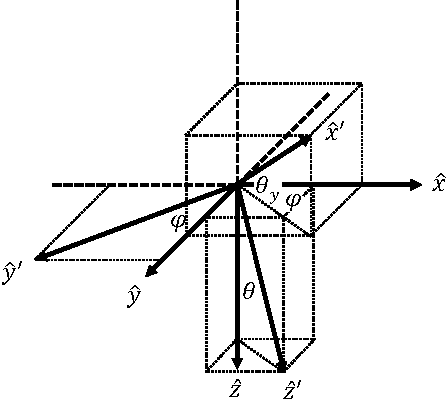
\includegraphics[scale=1.0]{coordinate_systems-crop.pdf}
\caption{Definition of the beam coordinate system $(\hat{x}', \hat{y}',
\hat{z}')$ and the target coordinate system $(\hat{x}, \hat{y}, \hat{z})$ by
tilt angle $\theta_y$ and rotation angle $\varphi$.}
\label{fig:coord}
\end{figure}   
%
The \textbf{initial direction} of the ions is defined by the nominal beam
direction (reference direction) and, optionally, by a beam 
divergence. The reference direction $\hat{z}'$ is defined by tilt angles 
$\theta_x$ and $\theta_y$ and a rotation angle $\varphi$ relative to the target 
coordinate system $(\hat{x}, \hat{y}, \hat{z})$, see Fig.~\ref{fig:coord}. To 
be more precise, the beam coordinate system $(\hat{x}', \hat{y}', \hat{z}')$ 
is obtained from the target coordinate system $(\hat{x}, \hat{y}, \hat{z})$ by 
first rotating the system about the $z$ axis by an angle $\varphi$, then
about the new $x$ axis by $\theta_x$ ($\theta_x=0$ in Fig.~\ref{fig:coord}), and 
finally about the new $y$ axis by $\theta_y$. In symbols:
%
\begin{equation}
    (\hat{x}, \hat{y}, \hat{z}) \rightarrow (\hat{x}', \hat{y}', \hat{z}'): 
        \mathbf{R}_z(\varphi) 
        \rightarrow \mathbf{R}_x(\theta_x)
        \rightarrow \mathbf{R}_y(\theta_y)
\end{equation}
%
Note that positive angles for rotations about the $z$ axis are defined so that
the positive $x$ axis is rotated towards the positive $y$ axis, for the $x$ axis
ao that the positive $y$ axis is rotated towards the positive $z$ axis, and for 
the $y$ axis so that the positive $z$ axis is rotated towards the positive $x$
axis. The corresponding rotation matrix is
%
\begin{equation}
    \mathbf{R} = \mathbf{R}_y(\theta_y) \mathbf{R}_x(\theta_x) 
        \mathbf{R}_z(\varphi) 
    \label{eq:rotation_matrix}
\end{equation}
Constructing the beam coordinate system from the target coordinate system is 
convenient for theoretical investigations. In practice, the beam coordinate
system is usually fixed in space, and the target is rotated. It is therefore
more convenient to construct the target coordinate system from the beam
coordinate system. To obtain the same relative orientations of the coordinate 
systems, the order of rotations has to be reversed, and the rotations have to
be performed in opposite directions.
In symbols:
%
\begin{equation}
    (\hat{x}', \hat{y}', \hat{z}') \rightarrow (\hat{x}, \hat{y}, \hat{z}): 
        \textbf{R}_y(-\theta_y)
        \rightarrow \textbf{R}_x(-\theta_x)
        \rightarrow \textbf{R}_z(-\varphi) 
\end{equation}
%

Using an axis of the rotated coordinate system for the next rotation defines
``intrinsic'' rotations. In some systems, rotations are always performed
about axes defined in the beam coordinate system. Such chained rotations
are called ``extrinsic''. It can be shown that extrinsic rotations are 
described by the same rotation matrix as intrinsic rotations 
(Eq.~\ref{eq:rotation_matrix}), if the rotations are interpreted as rotations 
of the target coordinate system relative to the beam coordinate system:
%
\begin{equation}
    (\hat{x}', \hat{y}', \hat{z}') \rightarrow (\hat{x}, \hat{y}, \hat{z}): 
        \textbf{R}_z(\varphi) 
        \rightarrow \textbf{R}_x(\theta_x)
        \rightarrow \textbf{R}_y(\theta_y) .
\end{equation}
%
While the individual rotations describe the rotation of the target coordinate
system relative to the beam coordinate system, the rotation matrix 
$\mathrm{R}$ describes the transformation from the target coordinate system
to the beam coordinate system like in the ``intrinsic'' rotations case.
Therefore, the user need not specify whether the rotations are extrinsic or
intrinsic.

Without beam divergence, the initial directions of all ions coincide with
the reference direction $\hat{z}'$ ($z$ axis of the beam coordinate system, 
cf.\ Fig.~\ref{fig:coord}). Considering beam divergence means to randomly 
select the ion’s direction vector on the unit sphere in the beam coordinate
system so that the probability per solid angle follows a given distribution 
centered around the reference direction. The beam divergence models may be 
chosen from two options: isotropic within a maximum rotation angle, and 
Gaussian with given standard deviations in $\hat{x}'$ and $\hat{y}'$ 
direction.

\begin{figure}[htbp]
\centering
\noindent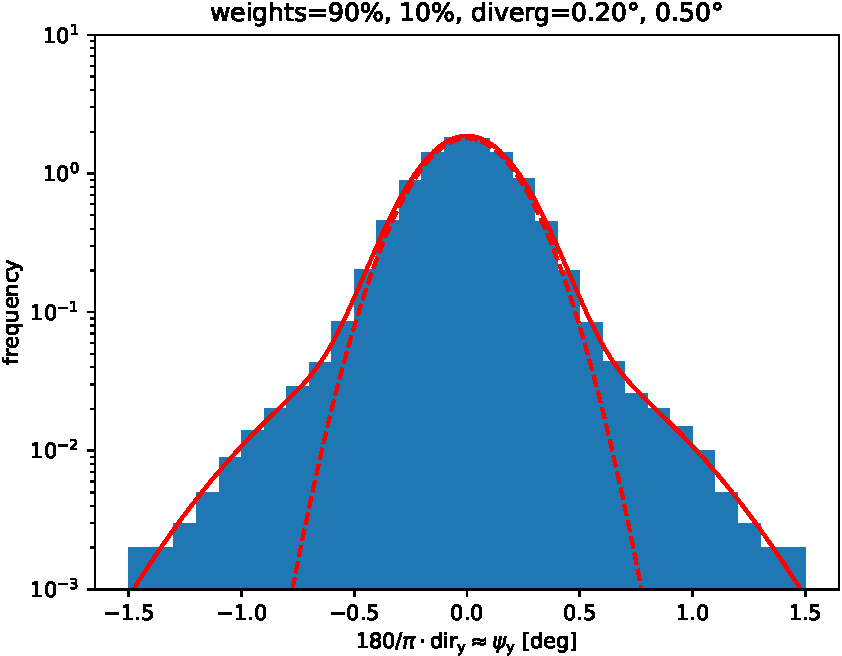
\includegraphics[scale=0.8]{diverg_y-crop.pdf}
\caption{Beam profile composed of two Gaussian functions (red line) and
histogram of angles \(\psi_\mathrm{y}\) generated by IMSIL.}
\label{fig:diverg}
\end{figure}  
%
More refined beam profiles or divergence distributions may be defined by
superposing partial beams using the \texttt{BEAM} index variable. An index
variable used on an input record specifies that the parameters on this record
apply to a particular object only, in this case to a partial beam. Each partial
beam may have a different beam profile and/or beam divergence. Ions are then
chosen with probabilities proportional to a specified beam weight from each of
the partial beams. An example for the superposition of two Gaussian beam
divergence distributions is shown in Fig.~\ref{fig:diverg}. Below is an excerpt
from an IMSIL input file that specifies this beam profile: 
%
\begin{verbatim}
   &IONS NAME='B' ENERGY=5000 DOSE=1e13 TILT=0 MODDIV=2 NION=10000 /
   &IONS BEAM=1 WEIGHT=0.9 DIVERG=0.1,0.2 /
   &IONS BEAM=2 WEIGHT=0.1 DIVERG=0.2,0.5 /
\end{verbatim}
%
Note that parameters that are specified on the first line, which does not have
the \texttt{BEAM} index variable, apply to both beams.

The \textbf{ion dose} may either be specified in ions per area in the $x$-$y$
plane (areal dose, units cm$^{-2}$), ions per length in $y$ direction (line
dose, units cm$^{-1}$), or ion count. The most natural choice among these
options depends on the dimensionality of the spatial histograms that are
computed: areal dose for 1-D, line dose for 2-D, and number doses for 3-D
histograms. However, other choices are possible, see Sections~\ref{s:his1d},
\ref{s:his2d}, and \ref{s:his3d}.

\begin{center}
\begin{tabular}{lll}
parameter \quad                   & IMSIL name & to be specified in record \\
\hline
internal starting point flag      & \texttt{LIINIT}    & \texttt{\&IONS} \\
ion name                          & \texttt{NAME}      & \texttt{\&IONS} \\
energy $E$                        & \texttt{ENERGY}    & \texttt{\&IONS} \\
atom mass $M$                     & \texttt{MASS}      & \texttt{\&ATOMS} \\
reference starting point          & \texttt{XINIT}     & \texttt{\&IONS} \\
                                  & \texttt{YINIT}     & \texttt{\&IONS} \\
                                  & \texttt{ZINIT}     & \texttt{\&IONS} \\
beam FWHM (FWHM$_x$, FWHM$_y$)    & \texttt{FWHM}      & \texttt{\&IONS} \\
tilt angle $\theta_x$             & \texttt{TILTX}     & \texttt{\&IONS} \\
tilt angle $\theta_y$   & \texttt{TILTY}=\texttt{TILT} & \texttt{\&IONS} \\
rotation angle $\varphi$          & \texttt{ROTATE}    & \texttt{\&IONS} \\
random rotation flag              & \texttt{RANROT}    & \texttt{\&IONS} \\
beam divergence model             & \texttt{MODDIV}    & \texttt{\&IONS} \\
beam divergence $(\psi_x,\psi_y$) & \texttt{DIVERG}    & \texttt{\&IONS} \\
beam index variable               & \texttt{BEAM}      & \texttt{\&IONS} \\
beam weight                       & \texttt{WEIGHT}    & \texttt{\&IONS} \\
dose                              & \texttt{DOSE}      & \texttt{\&IONS} \\
dose units                        & \texttt{DOSEUNITS} & \texttt{\&IONS} \\
number of simulated ions          & \texttt{NION}      & \texttt{\&IONS} \\
\end{tabular}
\end{center}
